%\documentclass[review]{elsarticle}
\documentclass[review, 3p, 11pt]{elsarticle}

\usepackage{lineno,hyperref}
\modulolinenumbers[5]

%\journal{Journal of \LaTeX\ Templates}

%%%%%%%%%%%%%%%%%%%%%%%
%% Elsevier bibliography styles
%%%%%%%%%%%%%%%%%%%%%%%
%% To change the style, put a % in front of the second line of the current style and
%% remove the % from the second line of the style you would like to use.
%%%%%%%%%%%%%%%%%%%%%%%

%% Numbered
%\bibliographystyle{model1-num-names}

%% Numbered without titles
%\bibliographystyle{model1a-num-names}

%% Harvard
%\bibliographystyle{model2-names.bst}\biboptions{authoryear}

%% Vancouver numbered
%\usepackage{numcompress}\bibliographystyle{model3-num-names}

%% Vancouver name/year
%\usepackage{numcompress}\bibliographystyle{model4-names}\biboptions{authoryear}

%% APA style
%\bibliographystyle{model5-names}\biboptions{authoryear}

%% AMA style
%\usepackage{numcompress}\bibliographystyle{model6-num-names}

%% `Elsevier LaTeX' style
\bibliographystyle{elsarticle-num}

\usepackage[pdftex]{graphicx}
%\usepackage[caption=false,font=footnotesize]{subfig}
%\usepackage{url}
%\usepackage{multirow}
%\usepackage{subfigure}
%\usepackage{caption}
\usepackage[caption=false]{subfig}
\usepackage{multicol}
\usepackage{amsmath}
\usepackage{color}
\usepackage{balance}
%\usepackage{hyperref}
%\setlength{\textfloatsep}{5pt}

\usepackage{algorithmic}
\usepackage{pseudocode}
\usepackage[linesnumbered,vlined,ruled]{algorithm2e}
\usepackage{threeparttable}
\usepackage{comment}
\usepackage{todonotes}
\usepackage{tabu}
\usepackage[justification=centering]{caption}
\usepackage{soul}
\usepackage{adjustbox}
\usepackage{commath}
\usepackage[acronym]{glossaries}
\usepackage{titlesec}
\usepackage[hidelinks=true]{hyperref}


%\usepackage{mathptmx}
%\DeclareCaptionFont{xipt}{\fontsize{11}{13}\mdseries}
%\usepackage[font=xipt,labelfont=bf]{caption}
%\usepackage[font=times]{caption}
%\usepackage[font=rm]{caption}

% \newfontfamily{\ubuntufont}{Times NeW Roman}
% \DeclareCaptionFont{ubuntu}{\ubuntufont}
\usepackage[font={footnotesize}]{caption}
%\usepackage{setspace}
%\doublespacing
%\setstretch{1.667} 

%\onehalfspacing
%\usepackage[left=3cm, right=3cm]{geometry}

% \setlength{\hoffset}{0.46cm} %2,54 + 0.46
% \setlength{\textwidth}{15cm} % text a4
%%%%%%%%%%%%%%%%%%%%%%%

\begin{document}

\begin{frontmatter}


\title{Screening Interacting Factors in IEEE 802.11ah Restricted Access Window Using Locating Arrays}



% \title{Elsevier \LaTeX\ template\tnoteref{mytitlenote}}
% \tnotetext[mytitlenote]{Fully documented templates are available in the elsarticle package on \href{http://www.ctan.org/tex-archive/macros/latex/contrib/elsarticle}{CTAN}.
% }

%% Group authors per affiliation:
% \author{\IEEEauthorblockN{Le~Tian\IEEEauthorrefmark{1}, Michael~Mehari\IEEEauthorrefmark{2}, Serena~Santi\IEEEauthorrefmark{1}, Steven~Latr\'e\IEEEauthorrefmark{1}\IEEEauthorrefmark{2},\\ Eli~De~Poorter\IEEEauthorrefmark{2}, Jeroen Famaey\IEEEauthorrefmark{1}}
% \IEEEauthorblockA{\IEEEauthorrefmark{1}University of Antwerp - imec, IDLab, Department of Mathematics and Computer Science, Belgium}
% \IEEEauthorblockA{\IEEEauthorrefmark{2}Ghent University - imec, IDLab, Department of Information Technology, Belgium}}

% \author[1]{Le Tian}
% \ead{le.tian@uantwerpen.be}

% \author[2]{Michael~Mehari}
% \ead{michael.mehari@ugent.be}

% \author[1]{Serena~Santi}
% \ead{Serena.Santi@uantwerpen.be}

% \author[1,2]{Steven~Latr\'e}
% \ead{Steven.Latre@uantwerpen.be}

% \author[2]{Eli~De~Poorter}
% \ead{eli.depoorter@ugent.be}

% \author[1]{Jeroen Famaey }
% \ead{jeroen.famaey@uantwerpen.be}


% \address[1]{University of Antwerp - imec, IDLab, Belgium}
% \address[2]{Ghent University - imec, IDLab, Belgium}


%\fntext[myfootnote]{Since 1880.}

%% or include affiliations in footnotes:
% \author[mymainaddress,mysecondaryaddress]{Elsevier Inc}
% \ead[url]{www.elsevier.com}

% \author[mysecondaryaddress]{Global Customer Service\corref{mycorrespondingauthor}}
% \cortext[mycorrespondingauthor]{Corresponding author}
% \ead{support@elsevier.com}

%\address[mymainaddress]{1600 John F Kennedy Boulevard, Philadelphia}
%\address[mysecondaryaddress]{360 Park Avenue South, New York}

\newacronym{raw}{RAW}{Restricted Access Window}
\newacronym{sumo}{SUMO}{Surrogate Modeling}
\newacronym{ap}{AP}{Access Point}
\newacronym{iot}{IoT}{Internet of Things}
\newacronym[plural=MCS,longplural={modulation and coding schemes}]{mcs}{MCS}{modulation and coding scheme}
\newacronym{rca}{RCA}{rate control algorithm}
\newacronym{moroa}{MoROA}{Model-Based RAW Optimization Algorithm}
\newacronym{taroa}{TAROA}{Traffic-Aware RAW Optimization Algorithm}
\newacronym{etaroa}{E-TAROA}{Enhanced Traffic-Aware RAW Optimization Algorithm}
\newacronym{rps}{RPS}{RAW Parameter Set}
\newacronym{edca}{EDCA/DCF}{Enhanced Distributed Channel Access and Distributed Coordination Function}
\newacronym{mtc}{MTC}{machine-type communication}
\newacronym{rpd}{RPD}{Relative Percent Difference}
\newacronym[plural=AIDs,longplural={association IDs}]{aid}{AID}{association ID}
\newacronym{csma}{CSMA/CA}{carrier-sense multiple access with collision avoidance}
\newacronym{rrse}{RRSE}{root-relative square error}
\newacronym{wpan}{WPAN}{wireless personal area network}
\newacronym{lpwan}{LPWAN}{low-power wide area network}
\newacronym{mac}{MAC}{media access control}






%\maketitle

\begin{abstract}
xx
\end{abstract}

\begin{keyword}
IEEE 802.11ah, restricted access window (RAW), surrogate model, real-time station grouping, multi-objective optimization
\end{keyword}

% IEEE 802.11ah; dense IoT networks; restricted access window (RAW); real-time RAW
% 22 optimization; dynamic traffic

\end{frontmatter}

\linenumbers

\glsresetall


\section{Introduction}

%Introduction to 802.11ah and all the decisions left open in the standard; potential parameters to study to optimize various performance metrics.

The \gls{iot} aims to provide connectivity among tens of billions of battery powered smart devices anytime and anywhere. Currently, there are two categories of low-power IoT communication technologies: \gls{wpan} and \gls{lpwan} technologies. However, as the transmission range of the WPAN technologies is too short (i.e., tens of meters) and throughput of the LPWAN technologies is too low (i.e., up to at most a few kilobits per
second), both of them can only be applied in a limited set of IoT scenarios. 

The new IEEE 802.11ah Wi-Fi standard, marketed as Wi-Fi HaLow, fills this gap.
It operates in the unlicensed sub-1 GHz frequency bands , and support transmission ranges from 100 m up to 1 km with data rates between 0.15 Mbps and 346.67 Mbps. Thus, IEEE 802.11ah has the potential to achieve much higher
transmission ranges than existing \gls{wpan} and much higher throughput than both \gls{wpan} and \gls{lpwan}
technologies. 

On the \gls{mac} layer, a novel channel access method, referred to as \gls{raw} is proposed to provide scalable
connectivity among large number of battery powered devices. \gls{raw} is based on station grouping and attempts to
reduce contention and collisions in highly dense deployments by dividing stations into groups and allowing channel access to one group at a time. Consequently, IEEE 802.11ah allows up to 8192 stations to connect to a single Access Point (AP). Figure \ref{fig:RAW} schematically depicts how \gls{raw} works. Specifically, the channel airtime is split into several intervals, some of which are assigned to RAW groups, while others are shared and can be accessed by all stations using the traditional \gls{edca}. Moreover, each RAW group consists of one or more equal-duration slots, among which the stations assigned to the RAW group are evenly split (using round robin assignment). The \gls{raw} related information is carried in the \gls{rps} element and broadcast by \gls{ap} at fixed interval. The \gls{rps} specifies the stations belonging to each group, the group start time, slot number and slot duration. For a more in-depth description of IEEE8 02.11ah and RAW, the reader is referred to existing literature ~\cite{Khorov2015a,Sensor2017, sensors80211ah}.

\begin{figure}[t]
  \centering
  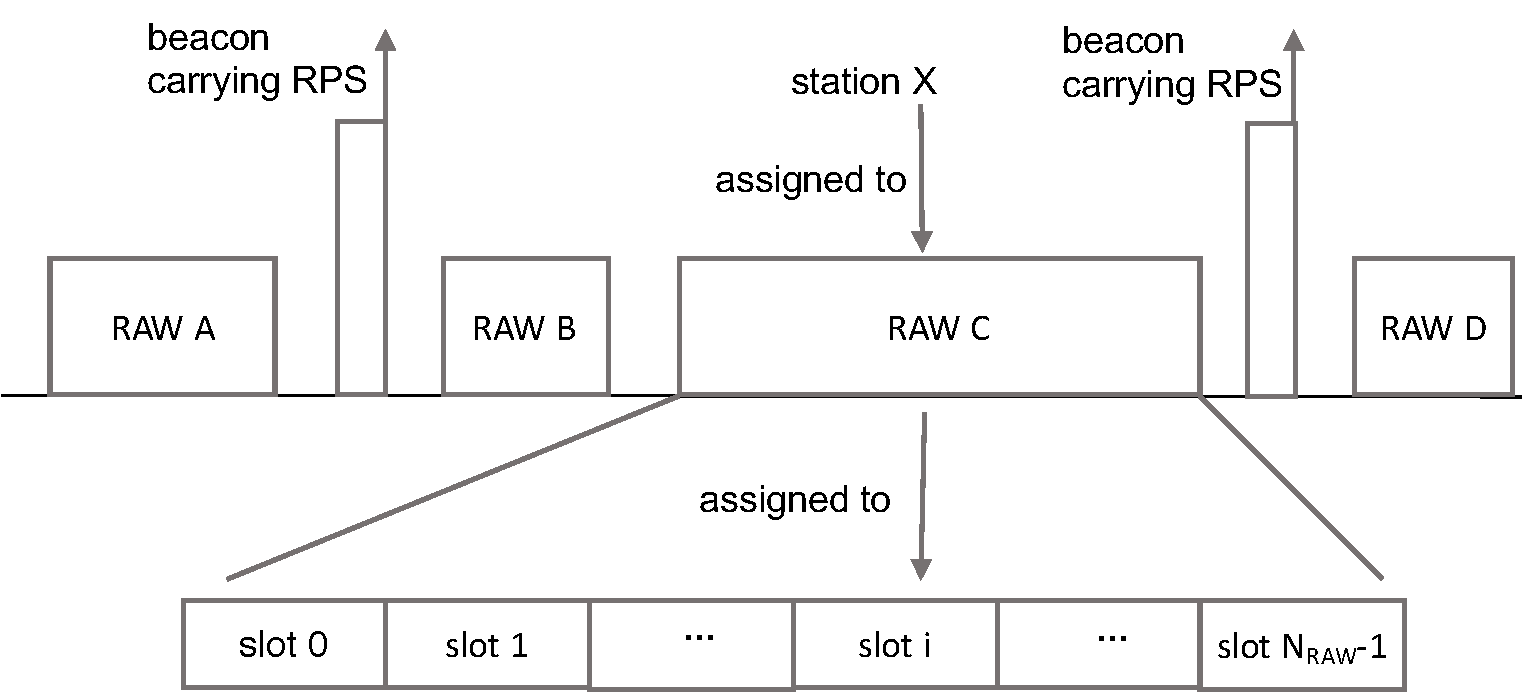
\includegraphics[width=0.8\columnwidth]{image/raw.pdf}
  \caption{\textbf{Schematic representation of the \gls{raw} mechanism}\label{fig:RAW}}
\end{figure}

The 802.11ah standard, however, does not specify how to configure the actual \gls{raw} grouping parameters. Previous research ~\cite{WoWMoM2016} has shown that the optimal \gls{raw} configuration depends on network-related parameters, such as the number of stations, traffic patterns, and network load~\cite{WoWMoM2016}. Incorrect configuration severely impacts throughput, latency and energy efficiency. However, it assumes homogeneous networks, i.e., all stations uses same \gls{mcs} and packet size, and stations are evenly divided into RAW groups. Moreover, some network-related parameters, such as beacon interval, channel width, station transmission queue size are not considered as fixed. 

As a step forward, in this paper, we evaluate the \gls{raw} performance with 17 network-related parameters, and use locating arrays to determine which parameters play a significant role in \gls{raw} optimization in terms of throughput and latency. In comparison to the research outlined above, the work presented in this paper is novel is two ways. First, it conducts a very comprehensive analysis on \gls{raw} performance, covering a quite broad range of network-related parameters, the obtained results can be considered as a guideline for designing \gls{raw} optimization algorithm for a variety of networks. Seconds, instead of analysis the network-related parameters exhaustively which requires \textcolor{red}{todo} experiments, the number of experiments is significant reduced by using locating arrays, only 304 (\textcolor{red}{todo\%}) experiments are used to study the \gls{raw} performance.

The remainder of this paper is structured as follows. Section~\ref{sec:parameters_selection} describes the evaluated network-related parameters and the selection of values for each parameter. 
Section~\ref{sec:locating_arrays} details the locating arrays method, how they are used for screening, and the new grouping idea to cope with the large number of values for some parameters. The experiments are described in Section~\ref{sec:setup}. Section~\ref{sec:evaluation} analysis the experiment results using locating arrays, determining the parameters which have significant roles in \gls{raw} optimization.
Finally, Section~\ref{sec:conclusion} offers conclusions and a short overview of future work.



% These works prove the strong
% correlation between network and traffic conditions on one
% hand, and the optimal RAW configuration on the other. This
% supports the hypothesis that there is a need for real-time RAW
% parameter optimization.

%evaluates \gls{raw} performance with all stations using same \gls{mcs} and packet size, the results

% In the past, several analytic models have been proposed to predict \gls{raw} performance~\cite{Khorov2015b,Wang2015}, and some algorithms has been proposed for RAW optimization~\cite{Chang2015,Ogawa2013, Qutab-Ud-Din2015, Sensor2017,Sensys2017, WoWMoM2018}. However, only a few network parameters are considered as variables. 




% As such, there is a need for \gls{raw} optimization algorithms that collect network-related information, and at the start of each beacon interval adapt the \gls{raw} configuration based on the current network conditions. 

% This is achieved using some sort model of the environment, which takes as input network conditions and a \gls{raw} configuration, and generates as output one or more performance metrics (e.g., throughput or energy consumption).




\section{IEEE 802.11ah \label{sec:802.11ah}}


\subsection{physical layer}
\subsection{MAC layer}



%\section{Mobility  \label{sec:mobility}}


\section{Experimental setup \label{sec:factors_selection}}

\subsection{ns-3 based IEEE~802.11ah simulator}

As there is no IEEE 802.11ah hardware available, All the experiments are performed using the extended version of IEEE 802.11ah ns-3 module \cite{WNS32018}. The implementation builds upon existing 802.11ah implementations in ns-3 \cite{wns32016}, it support a physical layer model for sub-1GHz radio communications and a subset of the new MAC layer features of the standard, such as \gls{raw} and its dynamic configuration interface, energy consumption model and TIM segmentation.

\subsection{mobility model}

In a simulation, in order to evaluate the effect of mobility on network performance, it is necessary to use a mobility model to accurately represent the movement of the nodes.
There are several mobility models that have been proposed and widely used in wireless network, such as 
Random Walk Mobility Model, Random Waypoint Mobility Model, Random Direction Mobility Model. There are also some other mobility models in which the node's decisions on movement depend upon the other node in the group. For a more detailed description of the mobility models, the reader is referred to existing literature \cite{camp2002survey}.


In the experiments, we consider the random Waypoint mobility model, which is supported by ns-3 simulator. Each node starts by pausing at time zero for the duration governed by the random variable "Pause". After pausing, the node will pick a new waypoint and a new random speed via the random variable "Speed", and will begin moving towards the waypoint at a constant speed. When it reaches the destination, the process starts over (by pausing). The new waypoint is picked via the ''RandomDiscPositionAllocator", which allocate random positions within a disc according to a given distribution for the polar coordinates of each node with respect to the provided center of the disc. The random variable "Pause" and "speed" are defined by their minimal values, maximal values, and random distribution types.


\subsection{IEEE~802.11ah network scenarios}


\begin{table}[t]
\centering
\renewcommand{\arraystretch}{1.2}
\scriptsize
\caption{PHY factors \label{tab:phy factors}}
\begin{tabular}{ll}
\hline
Frequency (Mhz)                & 868 \\
TX power (dBm)                 & 0    \\
TX/RX gain (dB)                & 0     \\
Noise Figure (dB)              & 6.8      \\  
Coding method                  & BCC \\
Propagation model              & Outdoor, \cite{globecom2017} \\ %, macro~\cite{Hazmi2012} \\
Error rate model               & YansErrorRate \\
\hline
\end{tabular}
\end{table}


We consider IoT scenario, where sensors periodically monitor the environment and send the resulting data to a server (via the AP). Different sensors may have different packet size, monitoring and transmission intervals. The transmission interval of sensors in an IoT network can follows different distributions. The default PHY layer factors used in our simulation are shown in Table~\ref{tab:factors}. Given the low-power nature of battery powered sensors, the PHY layer factors are configured based on the low-power 802.11ah radio hardware prototype developed by Ba et al.~\cite{Ba2016}, with a transmission power of 0~dBm, a gain of 0~dBi (for both sensor and AP), and noise figure of 6.8~dB. Stations are initially randomly placed around the AP in a circle, then move around following the pattern of the random Waypoint mobility model. The \gls{mcs} used for packet transmission are determined by the rate control method. Several rate control methods have been proposed and used on real devices for legacy IEEE~802.11 to select the appropriate MCS for packet transmission, for example, Arf \cite{arf1997},  Aarf \cite{aarf2004}, Onoe \cite{Onoe} and Minstrel \cite{minstrel2013}. In this paper, We aim to model instantaneous throughput with a single \gls{raw} group (i.e., one beacon interval at most),  \gls{mcs} changes at such a short time slot is are not expected. As such, we allow the stations to select the \gls{mcs} solely based on its distance to the \gls{ap}, i.e., choosing the MCS which can stably achieve the maximal throughput at a certain distance, as shown in Figure \ref{fig:dist-datarate}. 


\begin{figure}[t]
  \centering
  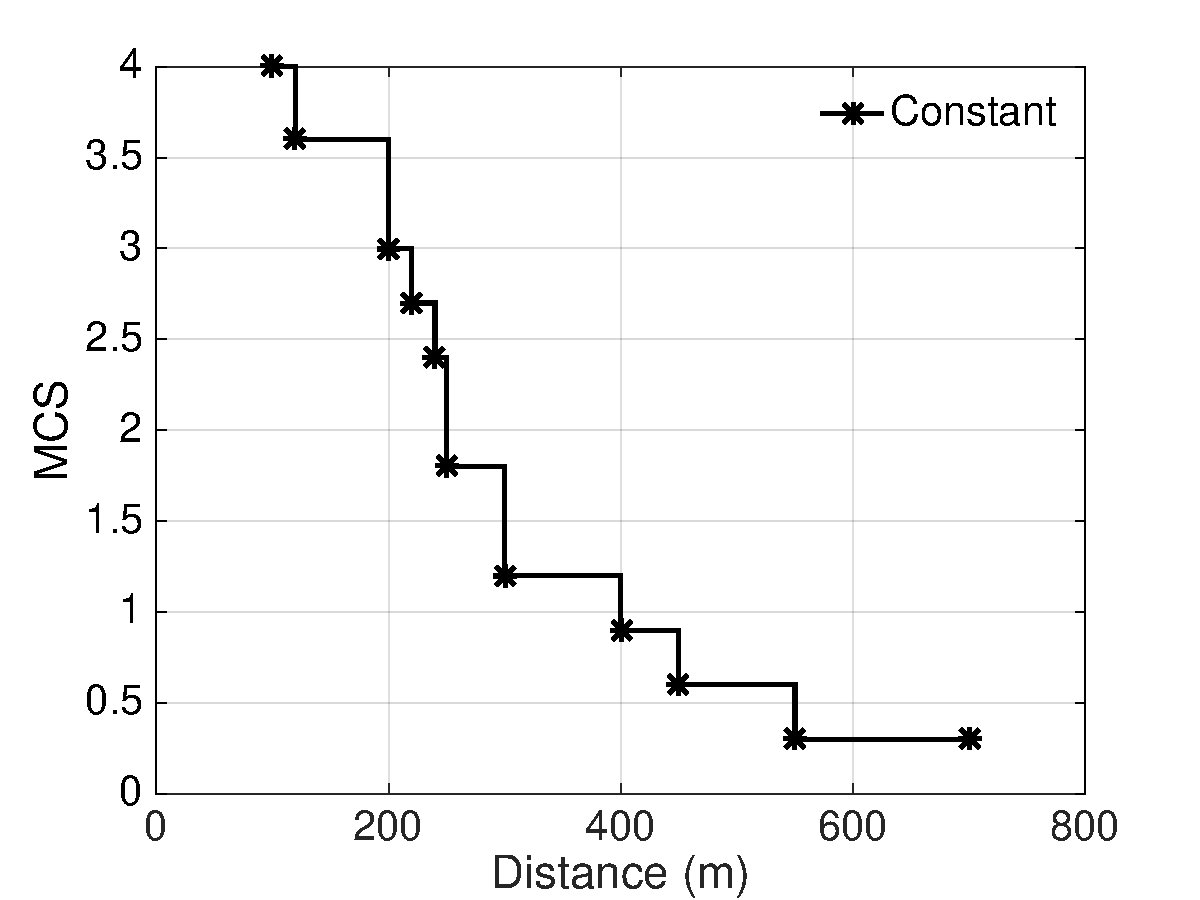
\includegraphics[width=0.45\textwidth]{image/distance-datarate}  \caption{\gls{mcs} as a function of the distance between a station and \gls{ap}. \label{fig:dist-datarate}}
\end{figure}

% \textcolor{red}{
% Some of the factors listed in table \ref{tab:ns3 factors} can be directly configured in the simulator, including network-related factors $\mathcal{B}$, $\mathcal{N}$, $l_q$,  $p_\textit{1M}$, $sta_\textit{dis}$ and $d_\textit{max}$, \gls{raw}-related factors $c_r$, $\textit{sl}_r$ and $n_r$. Based on factors  $s_\textit{dis}$, $s_\textit{min}$ and $s_\textit{max}$, a \textcolor{red}{new}  function is created to generate a packet size for each station. Similarly, another \textcolor{red}{new} function is created to generate a transmission interval for each station according to factors $i_\textit{dis}$, $i_\textit{min}$, and $i_\textit{max}$.\textcolor{red}{New function} is created to cluster stations and determines the \gls{raw} group duration based on the $g_r$ and $d_r$ factors, then configure the rps element via the \gls{raw} configuration interface.
% }



\subsection{Selected factors and values}

 Table \ref{tab:ns3 factors} lists the factors and their values used in experimentation. In total 19 factors are chosen, 14 of them are factors for network, the others are \gls{raw} related factors.


Five different beacon interval $\mathcal{B}$ are evaluated to assess the impact of beacon frame overhead on network performance. The station number varies from 25 to 2000 stations, with steps of 25, 50 and 250.
The channel width of IEEE 802.11ah ranges from 1 to  16 MHz, with only 1 and 2 MHz support mandatory. As we aim for \gls{iot} application, 1 and 2 MHz are evaluated in this experiment. The factors $p_\textit{1M}$ indicates the ratio of stations using 1 MHz channel width.
%$sta_\textit{dis}$ specifies whether stations are randomly located around \gls{ap} or stations are distributed along a circle.
$d_\textit{max}$ defines the maximal distance between stations and \gls{ap}. As the transmission range of IEEE 802.11ah is up to 1000 meters, we choose 21 values for this factor, ranging from 5 to 1000 meters, with a step size of 50. As the stations can adapt \gls{mcs} based on their distance to the \gls{ap}, this factor also implies a variety of \gls{mcs} used by stations.

Three factors $s_\textit{dis}$, $s_\textit{min}$ and $s_\textit{max}$ jointly determines the packet size of stations. The value \textit{uniform} for factors $s_\textit{dis}$ means the packet size follows uniform distribution on the interval [$s_\textit{min}$  $s_\textit{max}$]. While packet size follows gaussian distribution with a mean of ($s_\textit{min} + s_\textit{max}) / 2 $ \textit{gaussian} and a a standard deviation of 1.0. As the \gls{iot} scenarios are quite diverse, and they requires a variety of traffic types, similar to packet size distribution, we use factors $i_\textit{dis}$, $i_\textit{min}$  and $i_\textit{max}$ to generate different traffic types. The value \textit{uniform static} and \textit{gaussian static} for factors $i_\textit{dis}$ both indicate that stations send packets with a fixed time interval, while transmission interval follows uniform distribution on the interval [$i_\textit{min}$  $i_\textit{max}$] for \textit{uniform static}, and follows  gaussian distribution with a mean of ($i_\textit{min} + i_\textit{max})/ 2 $ \textit{gaussian} and a a standard deviation of 1.0 for \textit{gaussian static}. On the contrary, \textit{poisson variable} allows stations to transmit packets at a poisson rate of ($i_\textit{min} + i_\textit{max}) / 2 $. Since transmission queue length also has an impact on the network performance \cite{Duffy2007}, we investigate different transmission queue lengths $l_q$, ranging from 1 to infinite.  %The three different steps are designed in order to cope with \gls{raw} factors, explanation will be given in next paragraph.
For mobility, each station can randomly select its speed between [$v_{min}$, $v_{max}$], pause between [$p_{min}$, $p_{max}$]. Consider targeting applications of IEEE~802.11ah, a low speed of between 0.1 and 3 m/s is considered for $v_{max}$, and  a pause of between 0 and 200 seconds is considered for $p_{max}$. 


As indicated by factor $g_r$, Stations are split into $n_r$ distinct clusters (\gls{raw} group) based on a variety of distance metrics, i.e., \textit{MCS}, \textit{packet size}, \textit{TX time}, \textit{random} and \textit{distance}. Among them, \textit{TX time} means packet transmission time, and \textit{random} allows station to be randomly clustered. \gls{raw} groups ranging from 1 to 40 are evaluated with steps of 1, 2 and 5. %The three different steps are designed in such way in order to cover
The \gls{raw} group duration is determined by factor $d_r$, it assigns airtime among \gls{raw} groups in proportion to station number, packet transmission number and average packet transmission time when $d_r$ is set to \textit{stations} , \textit{packets} and \textit{TX time} respectively. When $d_r$ is \textit{uniform}, airtime is divided into \gls{raw} groups equally. The experiment support (non)cross slot boundary by setting $c_r$ to \textit{off}(\textit{on}). The number of RAW slots per group ranges from 1 to 64, where 1 is equivalent to \gls{csma}, and $64$ is maximal number of \gls{raw} slots supported by IEEE 802.11ah.


In comparison to scenarios considered in our previous research \cite{WoWMoM2016}, in this paper, a more broad range of factors are involved. The main difference are as follows. First, more realistic network scenarios are considered, stations can have different \gls{mcs}, packet size, transmission interval and transmission queue size, the stations can be parsley or densely located with same or different distance to \gls{ap}. Second, our experimentation evaluates a more diverse \gls{raw} grouping method, instead of dividing airtime and stations evenly among groups, stations assignment and \gls{raw} group duration varies based on different metrics. Table \ref{tab:ns3 factors} lists the factors and their values used in experimentation. In total 17 factors are chosen, 12 of them are factors for network, the others are \gls{raw} related factors.











\begin{table*}[t]
\centering
\renewcommand{\arraystretch}{1.2}
\scriptsize
\caption{Factors and levels used in experiment \label{tab:ns3 factors}}
\begin{tabular}{lll}
\hline
\textbf{Symbols}  & \textbf{Factors}            		 & \textbf{Levels}  \\
\hline
 $\mathcal{B}$ & Beacon interval (ms)            		        & 102.4, 204.8, 409.6, 1024, 2048  \\
 $\mathcal{N}$ & Station number              		        & 25, 50, 75, 100, 150, 200, $\dots$, 500, 750, $\dots$, 1750, 2000    \\
 $p_\textit{1M}$  & Bitrate probably 1 MHz                      & 0, 0.1, 0.2, $\dots$, 0.9, 1      \\  
 $sta_\textit{dis}$ & Station distribution         				& random \\
 $d_\textit{max}$ & Maximum station distance from the AP (m)       & 5, 50, 100, 150, $\dots$, 950, 1000 \\
 $s_\textit{dis}$ & Packet size distribution          & uniform, gaussian  \\
 $s_\textit{min}$ & Minimum packet size (bytes)       & 16, 32, $\dots$, 240, 256   \\
 $s_\textit{max}$ & Maximum packet size (bytes)       & MIN, $\dots$, 240, 256  \\
 $i_\textit{dis}$ & Packet arrival rate distribution  & uniform static, gaussian static, poisson variable\\
 $i_\textit{min}$ & Minimum packet arrival interval   & 1, 10, 30, 60, 600, 1200, 3600   \\
 $i_\textit{max}$ & Maximum packet arrival interval   & MIN, $\dots$, 3600  \\
 $l_q$ & Station transmission queue size (packets)   & 1, 10, 20, 50, 100, infinite   \\
  $\textit{v}_{min}$ & Minimum speed (m/s)     & 0.1 \\
 $\textit{v}_{max}$ & Maximum speed (m/s)     & 0.1,  0.2,  0.5,  1, 1.5,  2,  2.5, 3 \\
 $\textit{p}_{min}$ & Minimum pause (s)    & 0 \\
 $\textit{p}_{max}$ & Minimum pause (s)     & 0, 2, 5, 10, 20, 50, 100, 200  \\
 $g_r$ & RAW grouping strategy             & MCS, packet size, TX time, random, distance \\
 $n_r$ & Number of RAW groups              & 1, 2, 3, …, 9, 10, 12, 14, $\dots$, 20, 25, .., 40  \\
 $d_r$ & RAW group duration                & uniform, stations, packets, TX time  \\
 $c_r$ & Cross slot boundary               & on, off \\
 $\textit{sl}_r$ & Number of RAW slots per group     & 1, 2, 4, 6, 8, 16, 32, 48, 64 \\
\hline
\end{tabular}
\end{table*}


\section{Locating arrays \label{sec:locating_arrays}}


\section{Performance Evaluation and Discussion \label{sec:evaluation}}


\section{Conclusion and Future Work \label{sec:conclusion}}




\section*{Acknowledgement}
% Part of this research was funded by the Flemish FWO SBO S004017N IDEAL-IoT (Intelligent DEnse And Long range IoT networks) project. Serena Santi is funded by the Fund For Scientific Research (FWO) Flanders under grant number 1S82118N.


%\bibliographystyle{IEEEtran}
%\bibliography{references.bib}


% \bibnewpage 
% {
%   \doublespacing 
%   \bibliography{references.bib}
% }


%\begingroup\doublespacing

%\setstretch{1.667} 
%\doublespacing
\bibliographystyle{elsarticle-num}
\bibliography{references.bib}
%\endgroup






\end{document}